\documentclass[10pt,a4paper]{beamer}
\usepackage[T2A]{fontenc}
\usepackage[utf8]{inputenc}
\usepackage[english,russian]{babel}
\usepackage{amsmath}
\usepackage{amsfonts}
\usepackage{amssymb}
\usepackage{xcolor}
\usepackage{listings}
\usepackage[skip=10pt plus1pt]{parskip}

\lstset{tabsize = 2, escapeinside={№}{/№}}

\title{Создание системы выделения регистров для языка FCLang}
\author{Студент: Борисенков Никита Николаевич, 410 группа\\
Научный руководитель: c.н.с Кривчиков Максим Александрович}
\date{2025}

\begin{document}
\maketitle

\begin{frame}
    \frametitle{Введение}

    FCLang -- язык между ассемблером и C \cite{____2023}.

    В нём есть переменные, а значит под них нужно выделять регистры.

    Чтобы можно было проверить работоспособность алгоритма, так же сделан макет языка.

\end{frame}

\begin{frame}
    \frametitle{Введение}

    Предполагается для ручной оптимизации <<горячих>> участков кода.

    Должен иметь в себе систему типов.

    В качестве метаязыка/препроцессора используется язык Python.

    Есть переменные, которые ведут себя как именованные регистры.

    Хочется простую (небольшую по количеству кода) реализацию, чтобы было просто поддерживать.

\end{frame}

\begin{frame}
    \frametitle{Известные исследования. Раскраски графов}
    Раскраска графов предложена в \cite{chaitin_register_1981}.

    Переменным сопоставляются вершины. Рёбра есть, если пересекаются времена жизни.
    Цвета в раскраске соответствуют регистрам.

    Оптимальна в том смысле, что если выделение есть, то алгоритм его даст.

    NP-сложная задача.

\end{frame}

\begin{frame}
    \frametitle{Известные исследования. Раскраски графов}
    Если ограничивать класс графов, то есть более быстрые алгоритимы раскраски:

    Хордальные графы.
    В \cite{hutchison_register_2005} говорится, что большинство программ имеют такие.
    Есть алгоритм раскраски, линейный на хордальных графах.
\end{frame}

\begin{frame}
    \frametitle{Известные исследования. Раскраски графов}
    \textbf{Структурированные} программы имеют графы ограниченной древесной ширины.

    При фиксированном числе регистров есть линейный алгоритм раскраски графов \cite{hans_l_bodlaender_linear-time_1997}.

    Коэффициент линейной зависимости экспоненциально зависит от числа регистров. Если есть регистры разных видов, то сложность не может быть линейной. Есть полиномиальный алгоритм с показателем, зависящим от числа регистров.
\end{frame}

\begin{frame}[fragile]
    \frametitle{Известные исследования. Линейные сканирования}
    Линейное сканирование(linear scan) предложено в \cite{poletto_linear_1999}
    \begin{lstlisting}[language=python]
    def LinearScanRegisterAllocation():
        active = []
        for i in live_intervals: #№по возрастанию начала/№
            ExpireOldIntervals(i)
            if length(active) == R:
                SpillAtInterval(i)
            else
                i.register = free_registers.pop()
                active.insert(i) #№по убыванию конца/№
    def ExpireOldIntervals(i):
        for j in active: #№по возрастанию конца/№
            if j.endpoint >= i.startpoint:
                return
            active.remove(j) 
            free_registers.append(j.register)
    \end{lstlisting}

\end{frame}

\begin{frame}[fragile]
    \frametitle{Известные исследования. Линейные сканирования}
    \begin{lstlisting}[language=python]
    def SpillAtInterval(i):
        spill = active[-1]
        if spill.endpoint > i.endpoint:
            i.register =  spill.register]
            spill.location = new stack location
            active.remoce(spill)
            active.insert(i) #№по возрастанию конца/№
        else
            i.location = new stack locationk
    \end{lstlisting}

\end{frame}

\begin{frame}
    \frametitle{Известные исследования. Линейные сканирования}
    Развитие линейного сканирования -- Extended linear scan \cite{krishnamurthi_extended_2007}.

    Допускает вставление mov инструкций.

    Может давать результаты лучше раскраски графов.
\end{frame}

\begin{frame}
    \frametitle{Известные исследования. LLVM}
    Использует свой итеративный жадный алгоритм (greedy allocator)

    Основан на разрезании времени жизни и эвристиках по поводу того, какие переменные нужно держать на регистрах.

\end{frame}

\begin{frame}
    \frametitle{Постановка задачи}
    Нужно написать алгоритм выделения регистров с учётом особенностей FCLang.

    Особенности: нет автоматического выноса переменных в память, есть явные использования регистров.

    Нужно написать макет языка FCLang.

    Формально задачу выделения регистров можно сформулировать так: даны конечное множество переменных $V$,
    конечное множество регистров $R$ и программа $P = \{ c_i \subset V \sqcup R \}$.
    Определено отображение $live : V \rightarrow 2^P$ такое, что $v \in c \Rightarrow c \in live(v)$.
    Требуется построить отображение $reg : V \rightarrow R$ такое, что $\forall v, u \in V, v \neq u, live(v) \cap live(u) \neq \emptyset \Rightarrow reg(v) \neq reg(u)$
    и $\forall v \in V, r \in R \left(\exists c \in live(v), r \in c \Rightarrow reg(v) \neq r \right)$, если это возможно, а иначе сообщить о невозможности.
\end{frame}

\begin{frame}
    \frametitle{Выбранный алгоритм}

    За основу взято линейное сканирование.

    Причины выбора:
    \begin{itemize}
        \item линейная сложность без большого коэффициента
        \item не требуется большого количества памяти
        \item простота реализации
        \item программы могут быть произвольными, поэтому алгоритмы опирающиеся на хордальность или ограниченную древесную ширину не подходят.
    \end{itemize}

    К нему дополнительно добавлена проверка на то, а можно ли выделить регистр переменной.


\end{frame}

\begin{frame}[fragile]
    \frametitle{Проблема}

    Выбранный алгоритм не всегда даёт результат когда это возможно
    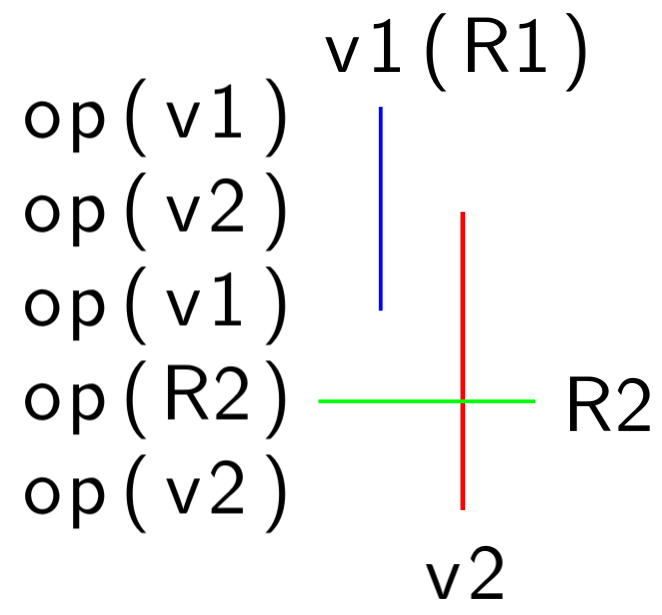
\includegraphics[scale=0.4]{fail_when_possible.png}
\end{frame}

\begin{frame}[fragile]
    \frametitle{Проблема}
    \begin{figure}[h]
        \begin{minipage}[h]{0.47\linewidth}
            \begin{tabular}{*{6}{|c}|}
                \hline
                & r1 & r2 & r3 & r4 & r5\\
                \hline
                v1 & x& & x& & \\
                \hline
                v2 & x& x& x& & \\
                \hline
                v3 & & & & x&x \\
                \hline
                v4 & &x & & x&x \\
                \hline
                v5 & x& x&x & & \\
                \hline
            \end{tabular}
        \end{minipage}
        \begin{minipage}[h]{0.47\linewidth}
            $\text{perm}\left(
            \begin{array}{*{5}{c}}
                0&1&0&1&1\\
                0&0&0&1&1\\
                1&1&1&0&0\\
                1&0&1&0&0\\
                0&0&0&1&1\\
            \end{array}\right) \overset{?}{=} 0$
        \end{minipage}

    \end{figure}

\end{frame}

\begin{frame}[fragile]
    \frametitle{Макет языка. Описание}
\begin{lstlisting}
<program>       №$\rightarrow$/№ <block declaration>№$^{*}$/№ <block>№$^{*}$/№
<block>         №$\rightarrow$/№ <block start> <block part>№$^{*}$/№
                                     <block exit>
<block start>   №$\rightarrow$/№ <block begin> <variable as input>№$^{*}$/№
<block exit>    №$\rightarrow$/№ pass_control
                   <block name and variables to pass>
<block part>    №$\rightarrow$/№ <variable definition> 
                    | <instruction>
                    | <conditional exit>
<conditional exit> №$\rightarrow$/№ condition_pass <condition>
                     <block name and variables to pass>
\end{lstlisting}

\end{frame}

\begin{frame}[fragile]
    \frametitle{Макет языка. Пример}
    \begin{lstlisting}[language=Python]
hello = "Hello World!\n"

main = Def()
loop = Def()
print = Def()
finale = Def()
with main:
    number = Variable()
    Mov(number, len(hello) - 1)
    pass_control((loop , [number]))

with loop:
    number = Variable()
    number.set_as_input()
    Add(number, -1)
    condition_pass(Flag.Zero, False, (print, [number]))
    pass_control((finale, []))

    \end{lstlisting}

\end{frame}

\begin{frame}[fragile]
    \frametitle{Макет языка. Пример}
    \begin{lstlisting}[language=Python]
with print:
    number = Variable()
    offset = Variable()
    offset.set_as_input()
    Mov(number, hello)
    Add(number, offset)

    write(1, number, byte_length(hello))
    pass_control((loop, [offset]))

with finale:
    exit(0)
    \end{lstlisting}

\end{frame}

\begin{frame}[fragile]
    \frametitle{Макет языка. Пример}
    \begin{lstlisting}[language=Python]
def syscall(syscall_id: Syscalls, *args):
    Mov(RAX, syscall_id)
    registers = [RDI, RSI, RDX, R10, R8, R9]
    for i in range(len(args)):
        if isinstance(args[i], Variable):
            try:
                Bind(args[i], registers[i])
            except Exception:
                Mov(registers[i], args[i])
        else:
            Mov(registers[i], args[i])
    Syscall()
\end{lstlisting}
\end{frame}

\begin{frame}
    \frametitle{Как это можно развить}
    Добавить SMID регистры.

    Нынешняя реализация не позволят использовать части регистра.
    С векторными регистрами это необходимо.
\end{frame}

\begin{frame}
    \frametitle{Заключение}
    В этой работе был реализован алгоритм выделения регистров.
    Был создан макет языка, который показывает работоспособность этого алгоритма.
\end{frame}
\bibliographystyle{apalike}
\bibliography{fclang_register_allocation}
\end{document}
